\documentclass[a4paper,10pt]{article}
\usepackage[utf8]{inputenc}
\usepackage{graphicx}

%opening
\title{Nonlinear interaction in Barotropic Vorticity Equation on the sphere}
\author{P. Peixoto}

\begin{document}

\maketitle

\begin{abstract}
Preliminar presentation of simulation results.
\end{abstract}

\section{Test case 1}

This test case includes in the initial condition energy on modes $(2,1)$, $(3,3)$, $(4,2)$, as shown in figure \ref{fig:tc-3-3-diagram}. 

\begin{figure}[h!]
\centering
 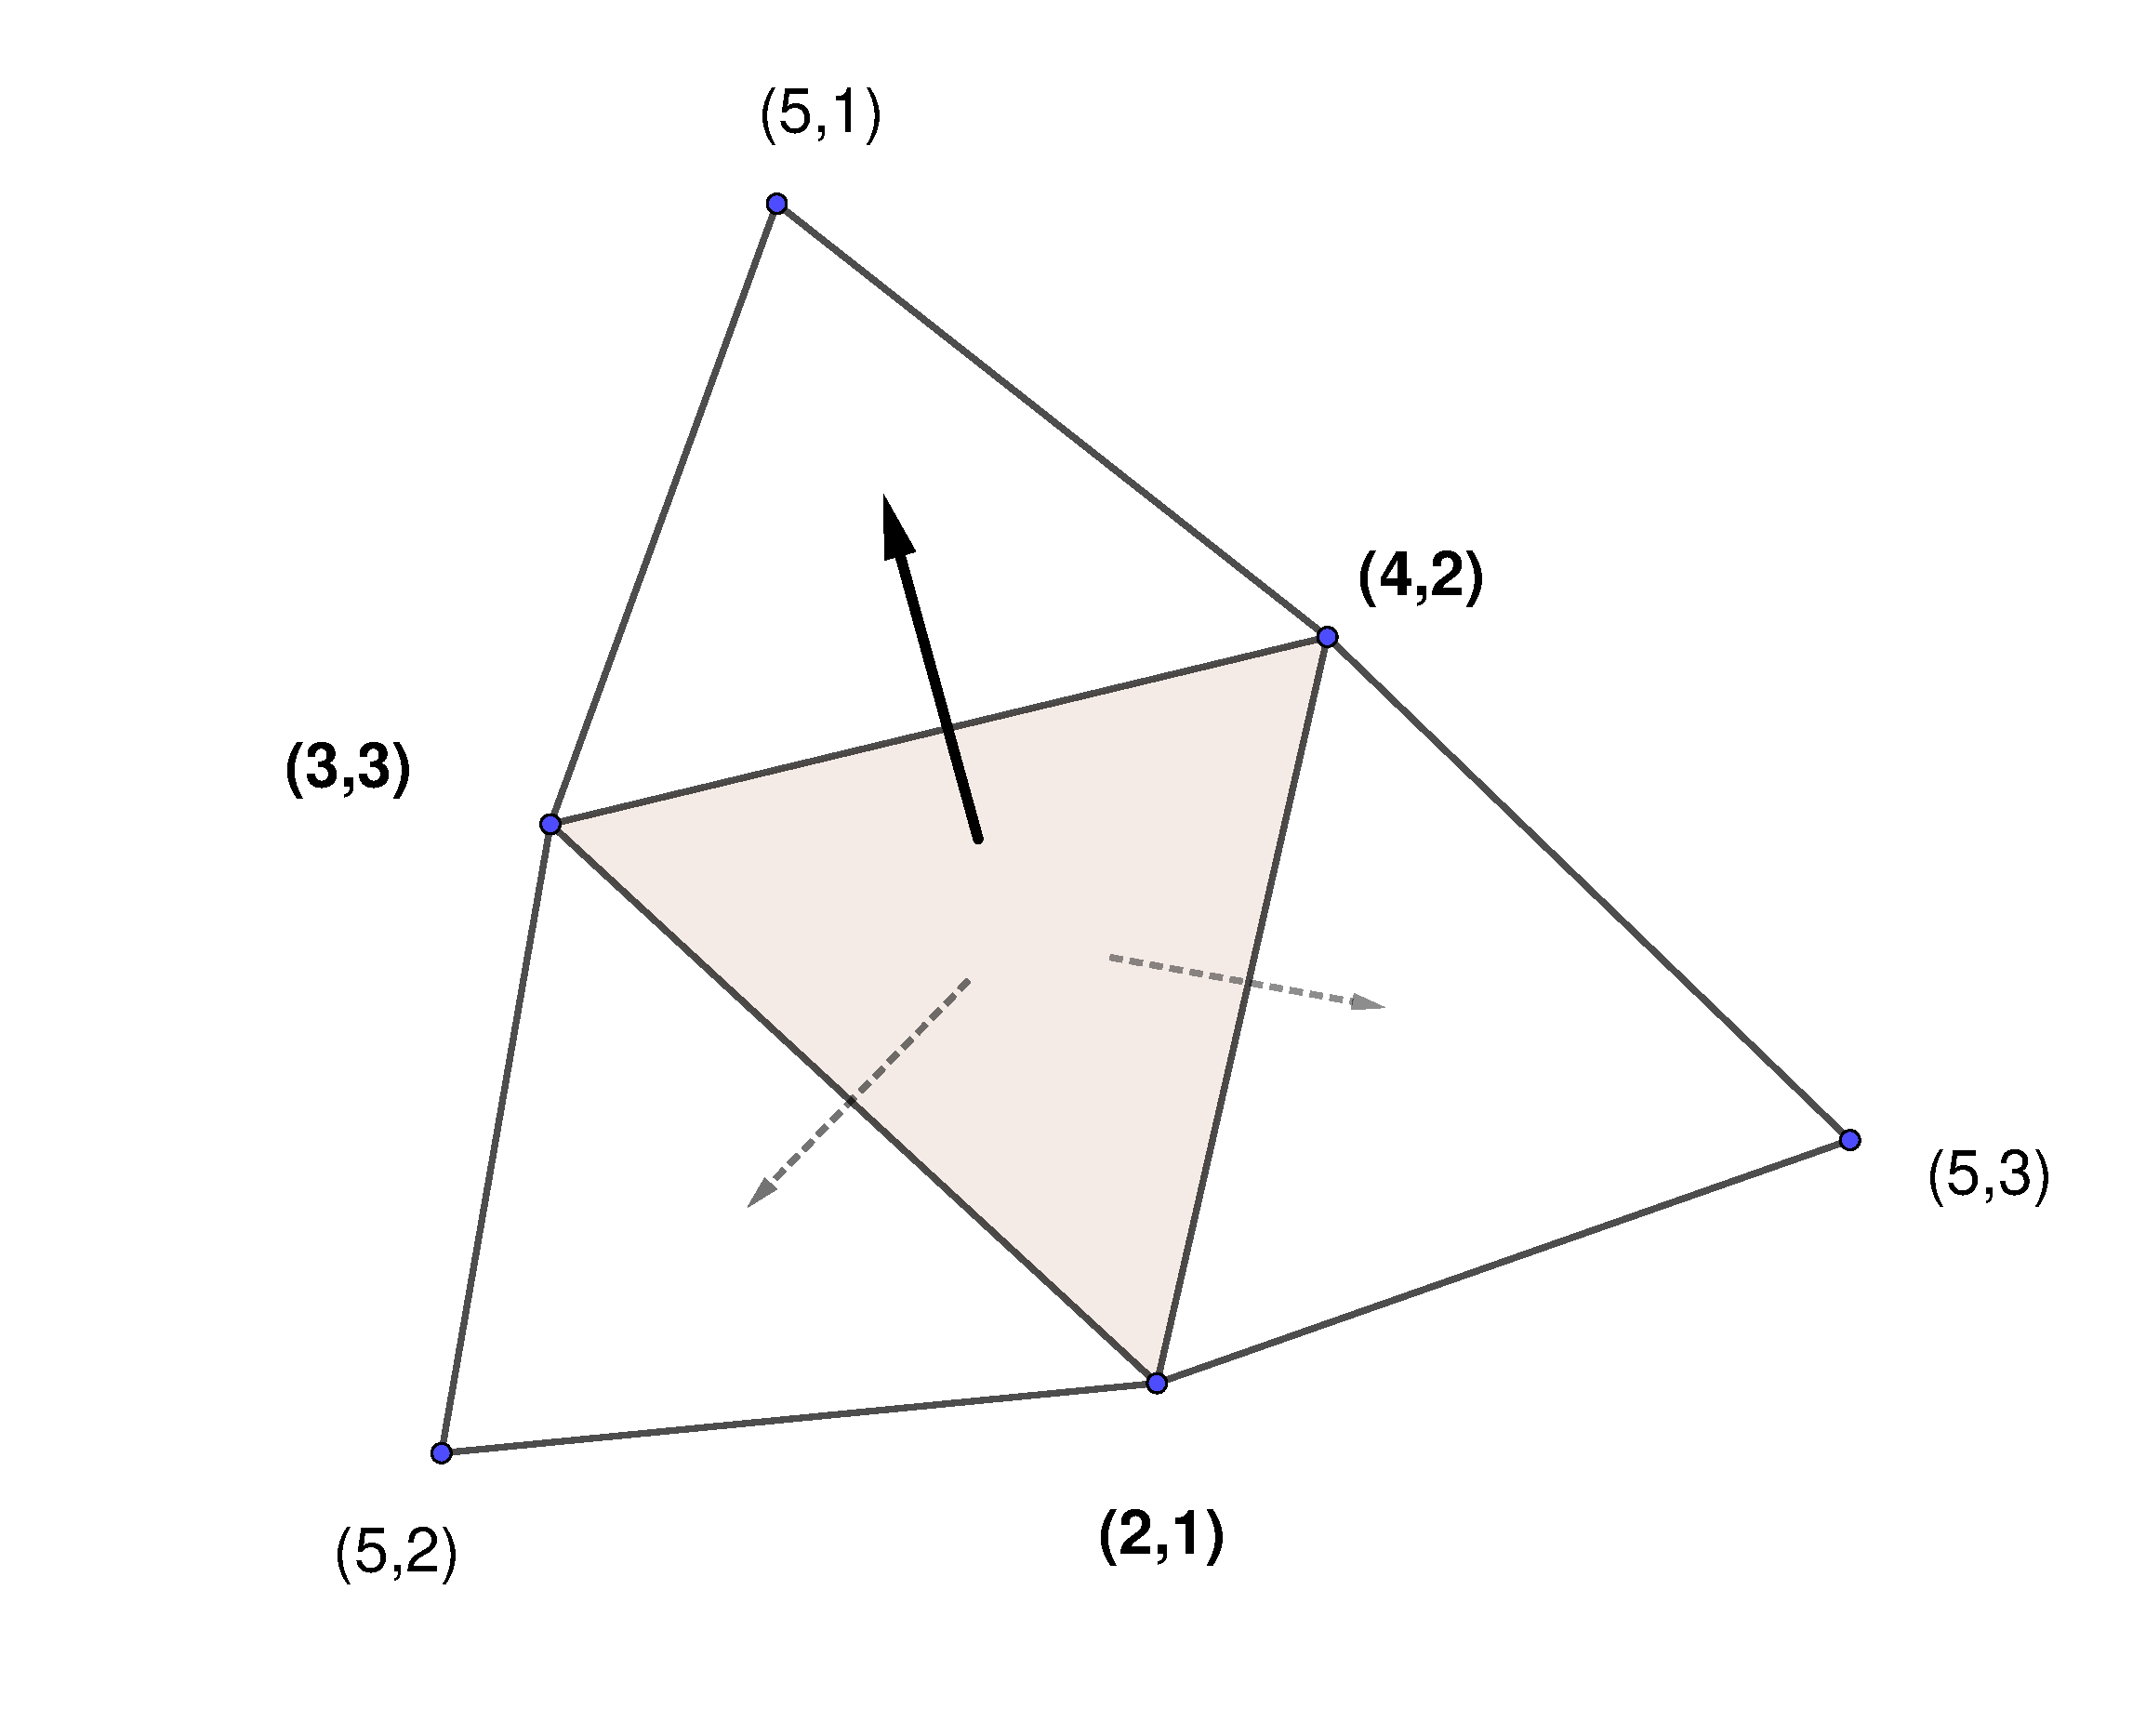
\includegraphics[scale=0.3]{figs/Nonlinear interaction diagram-TC-3-3.pdf}
 \label{fig:tc-3-3-diagram}
 \caption{Ilustration of triplet interaction for test case 1. Modes described as $(n,m)$.}
\end{figure}


\begin{figure}
\centering
 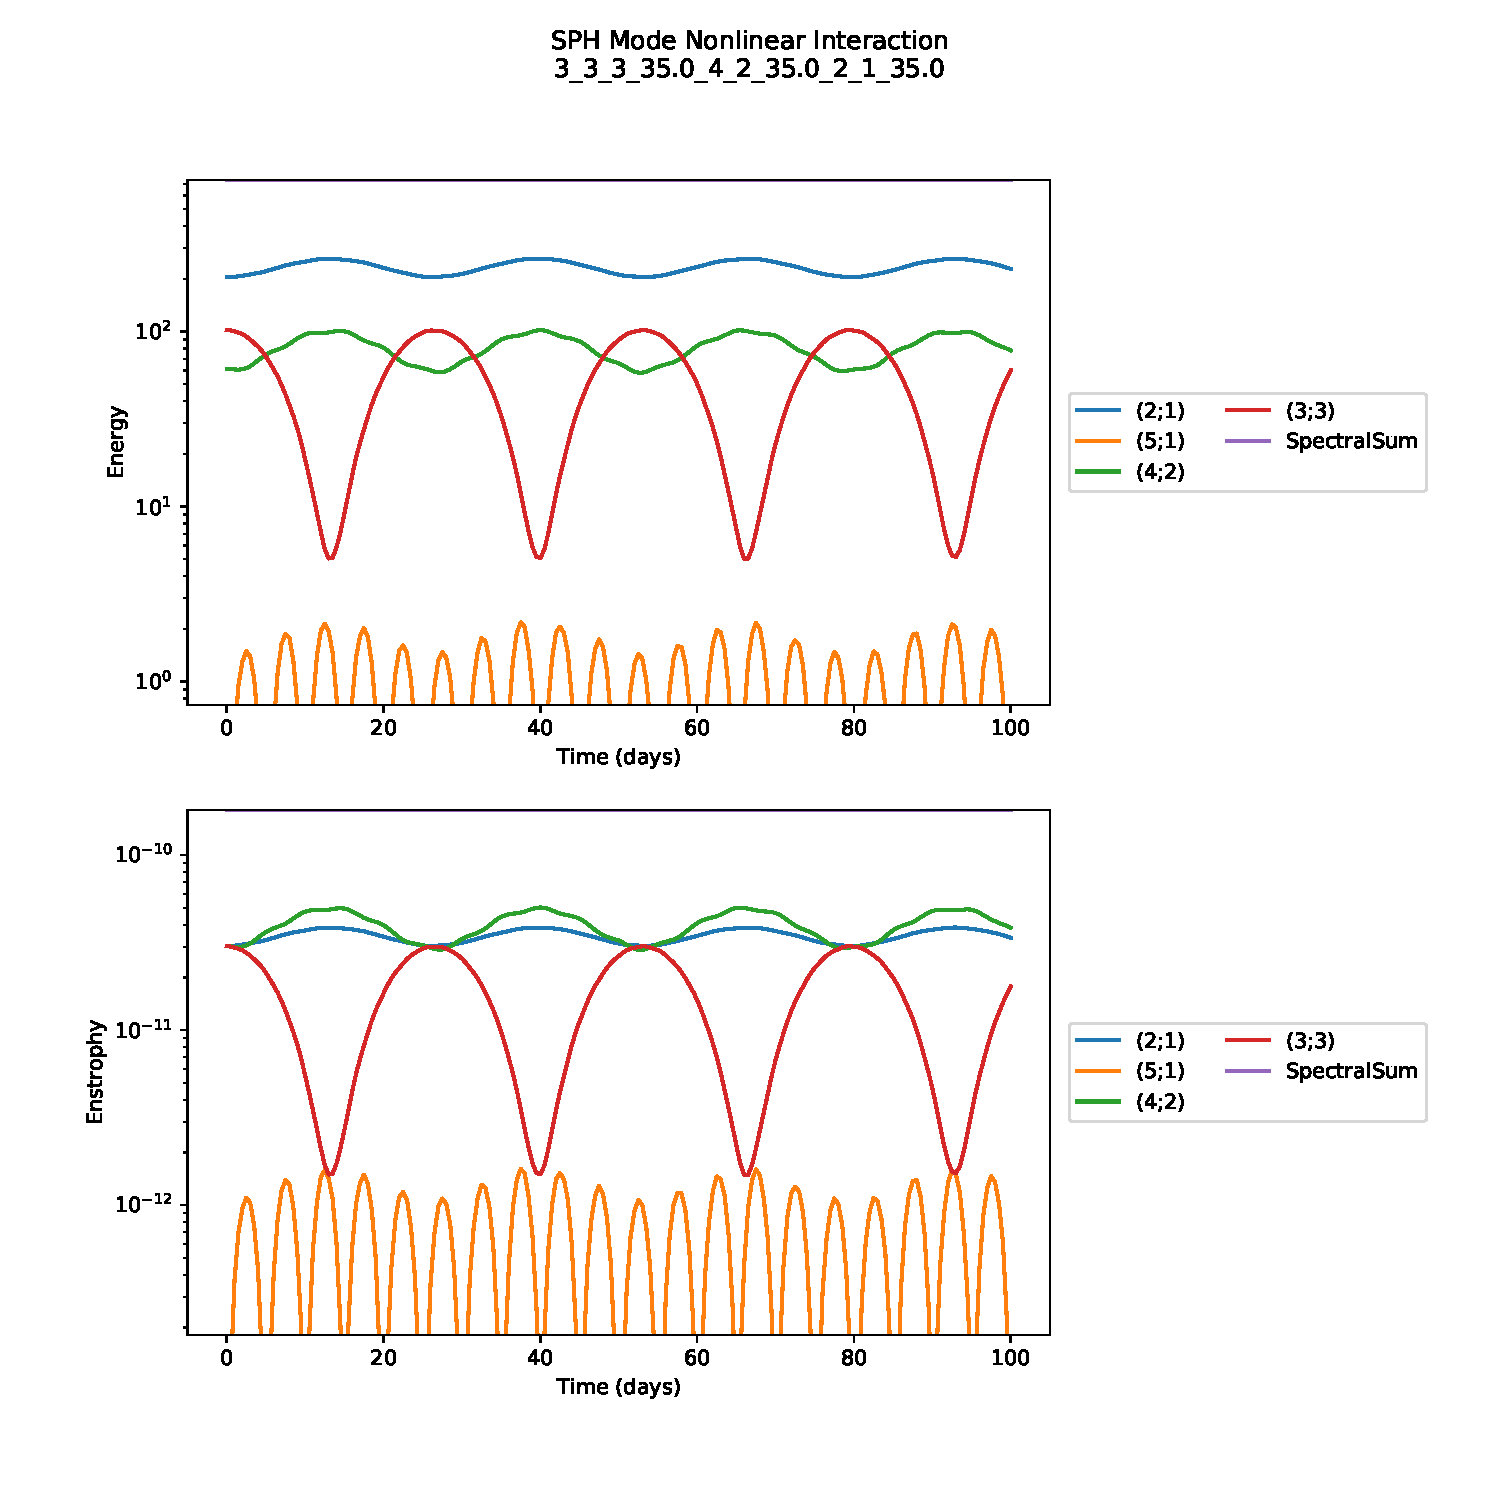
\includegraphics[scale=0.6]{figs/mode_evol_TC2_3-3-alpha35.pdf}
 \label{tc1-alpha35}
 \caption{Evolution of energy in specific modes considering initial condition with $\alpha=35$ on modes $(2,1)$, $(3,3)$, $(4,2)$.}
\end{figure}


\begin{figure}
\centering
 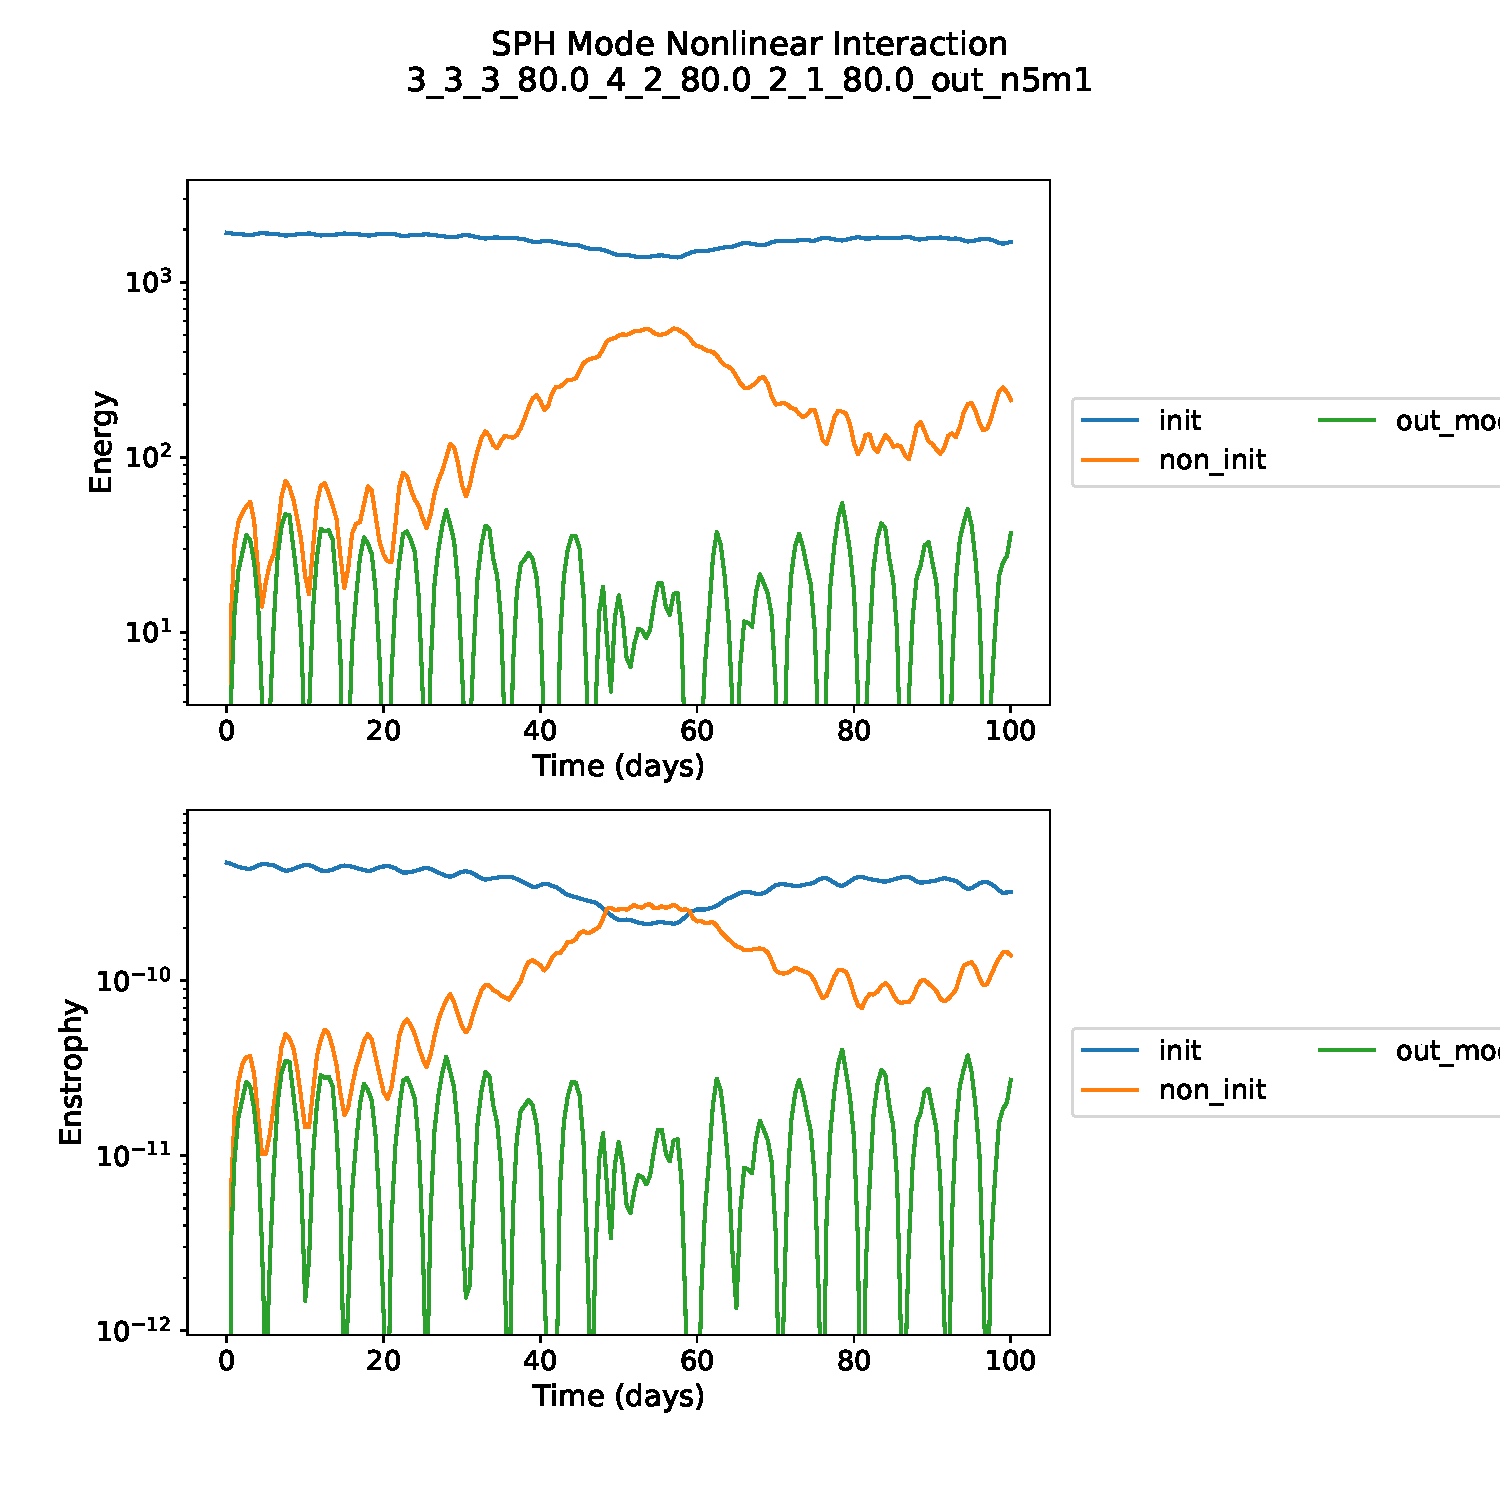
\includegraphics[scale=0.6]{figs/out_n5m1-alpha80.pdf}
 \label{tc1-alpha80}
 \caption{Evolution of energy in specific modes considering initial condition (init) with $\alpha=80$ on modes $(2,1)$, $(3,3)$, $(4,2)$. Non-init are all other modes not on initial condition and out-mode is mode $(5,1)$.}
\end{figure}

\begin{figure}
\centering
 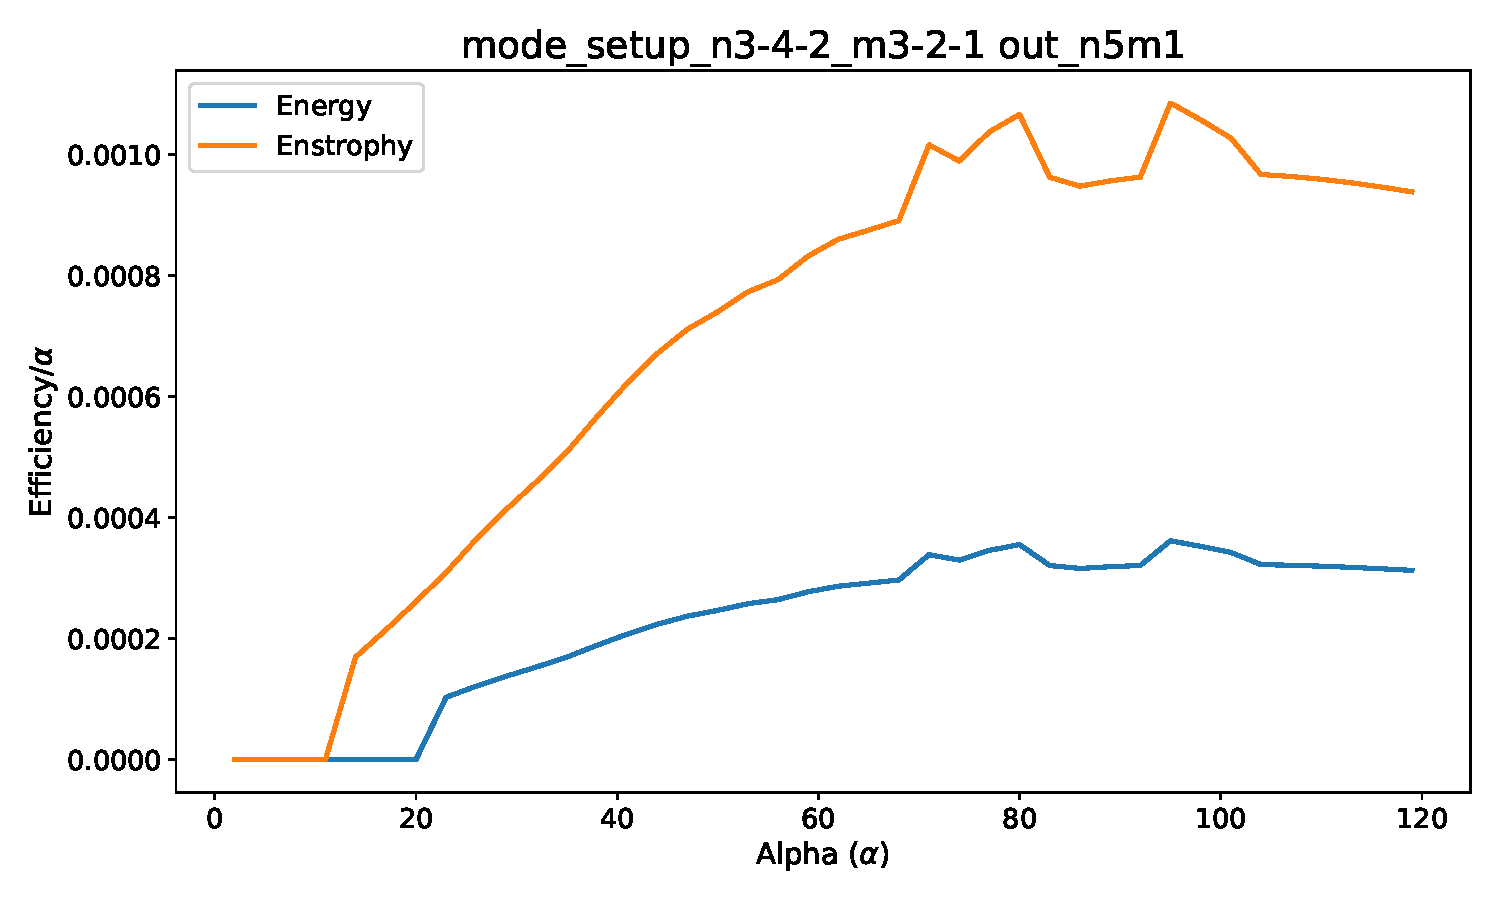
\includegraphics[scale=0.4]{figs/mode_setup_n3-4-2_m3-2-1_out_n5m1.pdf}
 \label{tc1-eficiency}
 \caption{Efficiency for test case with initial condition in modes modes $(2,1)$, $(3,3)$, $(4,2)$ monitoring the energy transfer to mode $(5,1)$.}
\end{figure}



\clearpage 

\section{Test case 2}


This test case includes in the initial condition energy on modes $(3,1)$, $(5,4)$, $(7,3)$, as shown in figure \ref{fig:tc-9-2-diagram}. 

\begin{figure}[h!]
\centering
 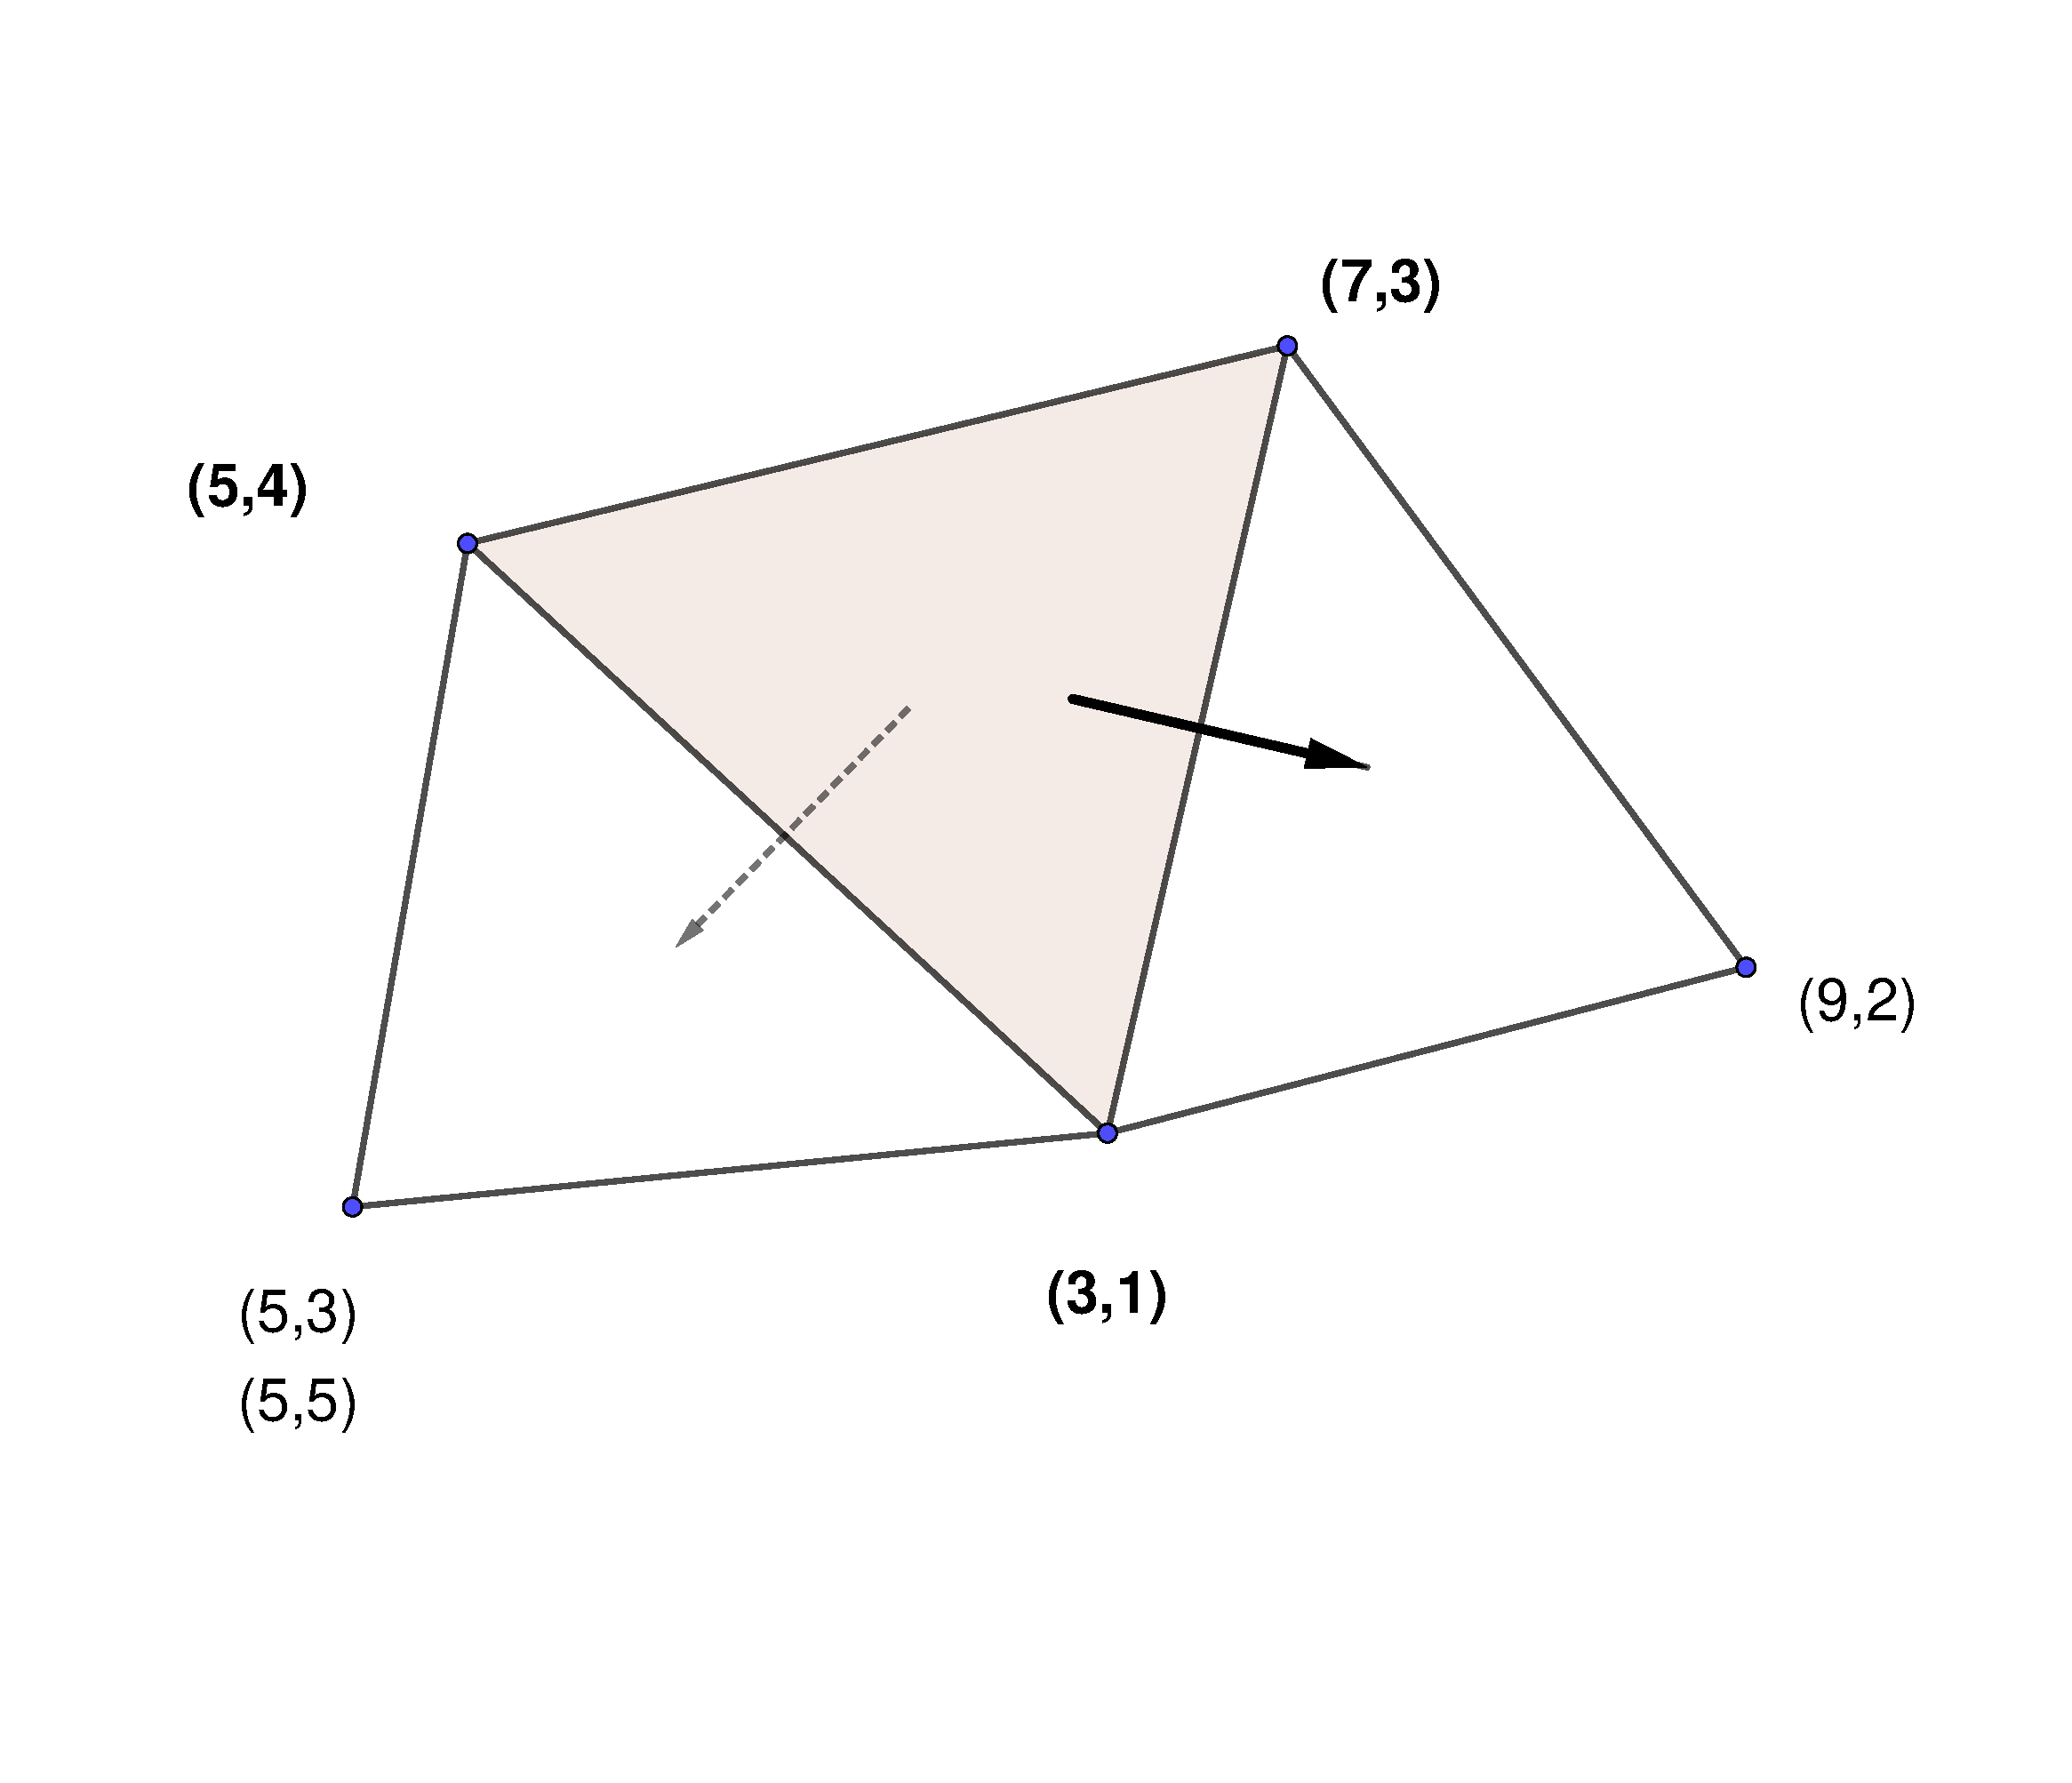
\includegraphics[scale=0.3]{figs/Nonlinear interaction diagram-TC-9-2.pdf}
 \label{fig:tc-9-2-diagram}
 \caption{Ilustration of triplet interaction for test case 2. Modes described as $(n,m)$.}
\end{figure}



\begin{figure}
\centering
 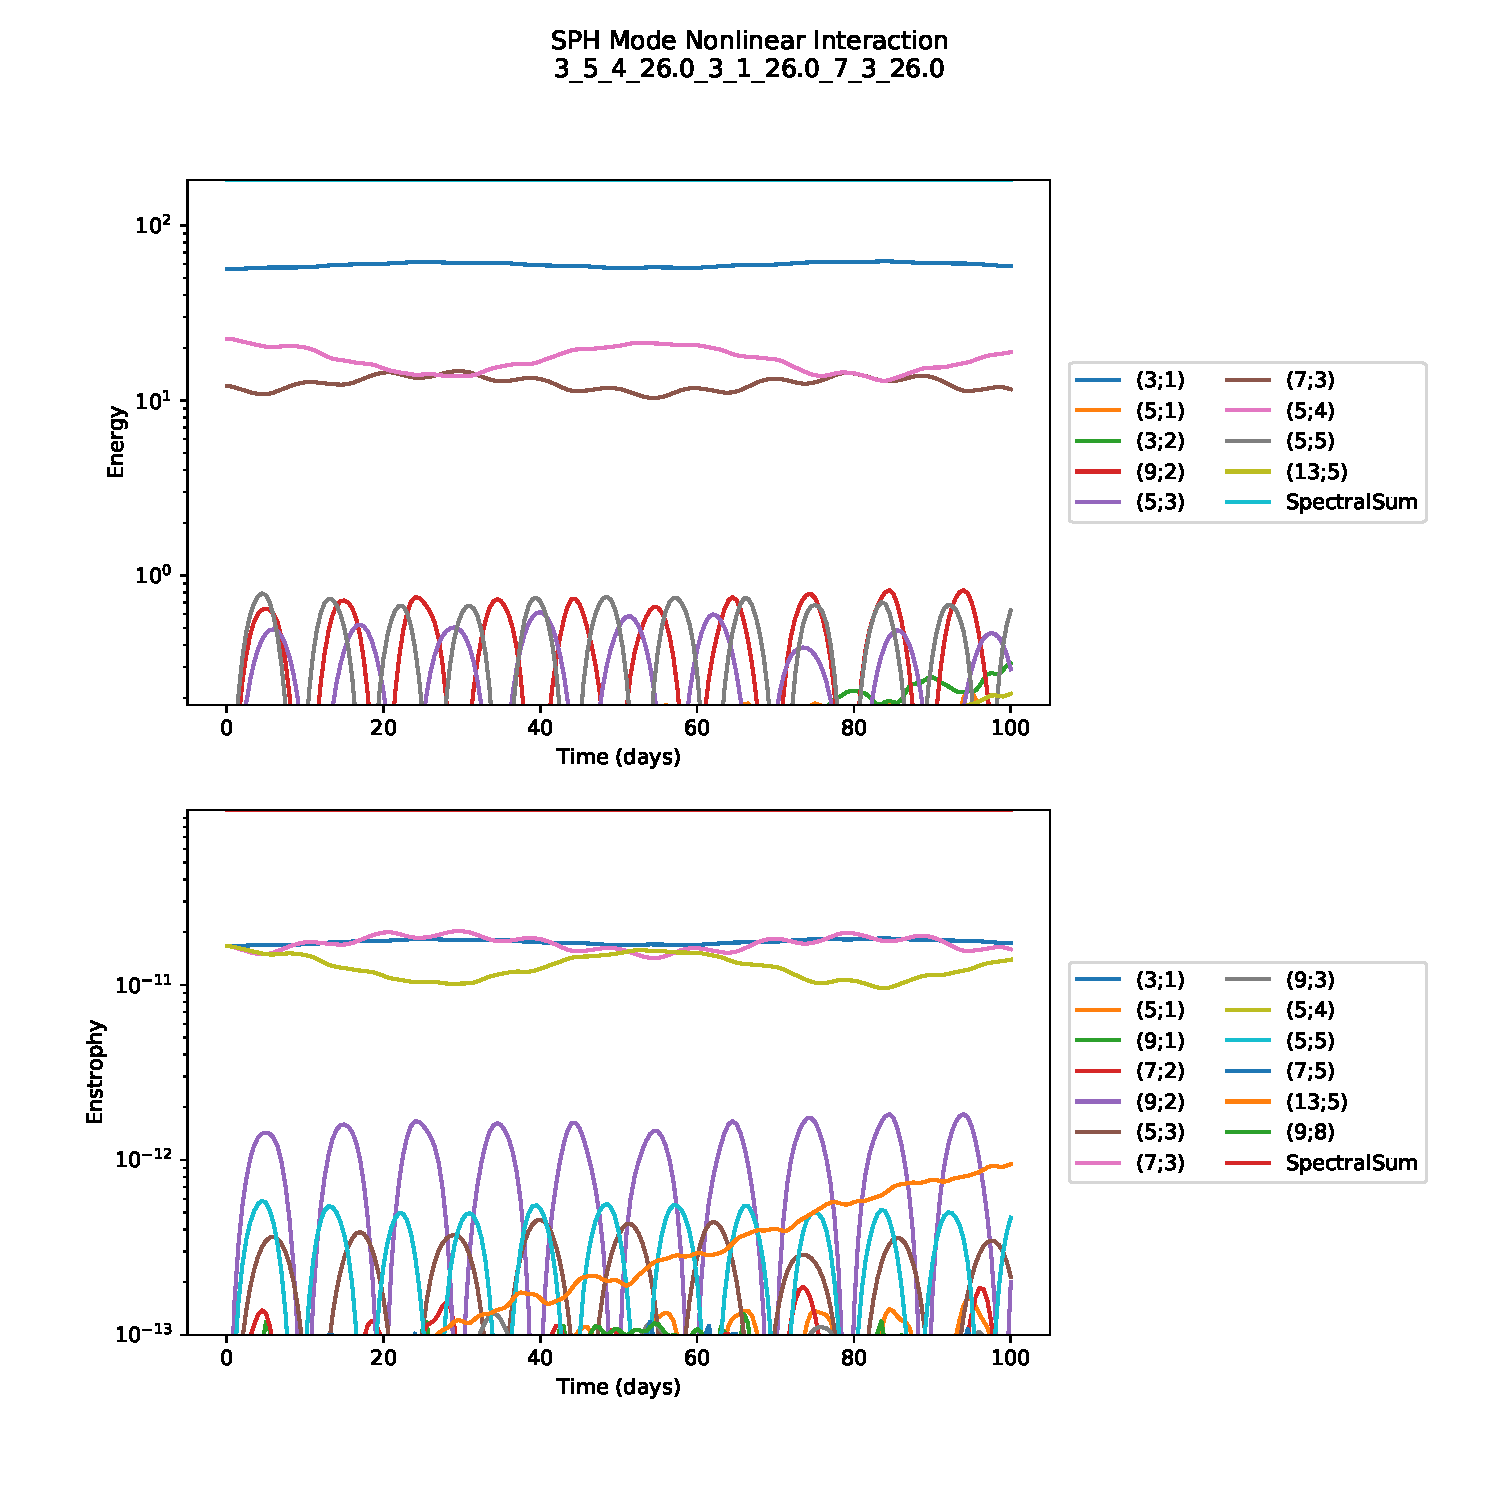
\includegraphics[scale=0.6]{figs/mode_evol_TC2-9-2.pdf}
 \label{tc2-alpha26}
 \caption{Evolution of energy in specific modes considering initial condition with $\alpha=26$ on modes $(3,1)$, $(5,4)$, $(7,3)$.}
\end{figure}



\begin{figure}
\centering
 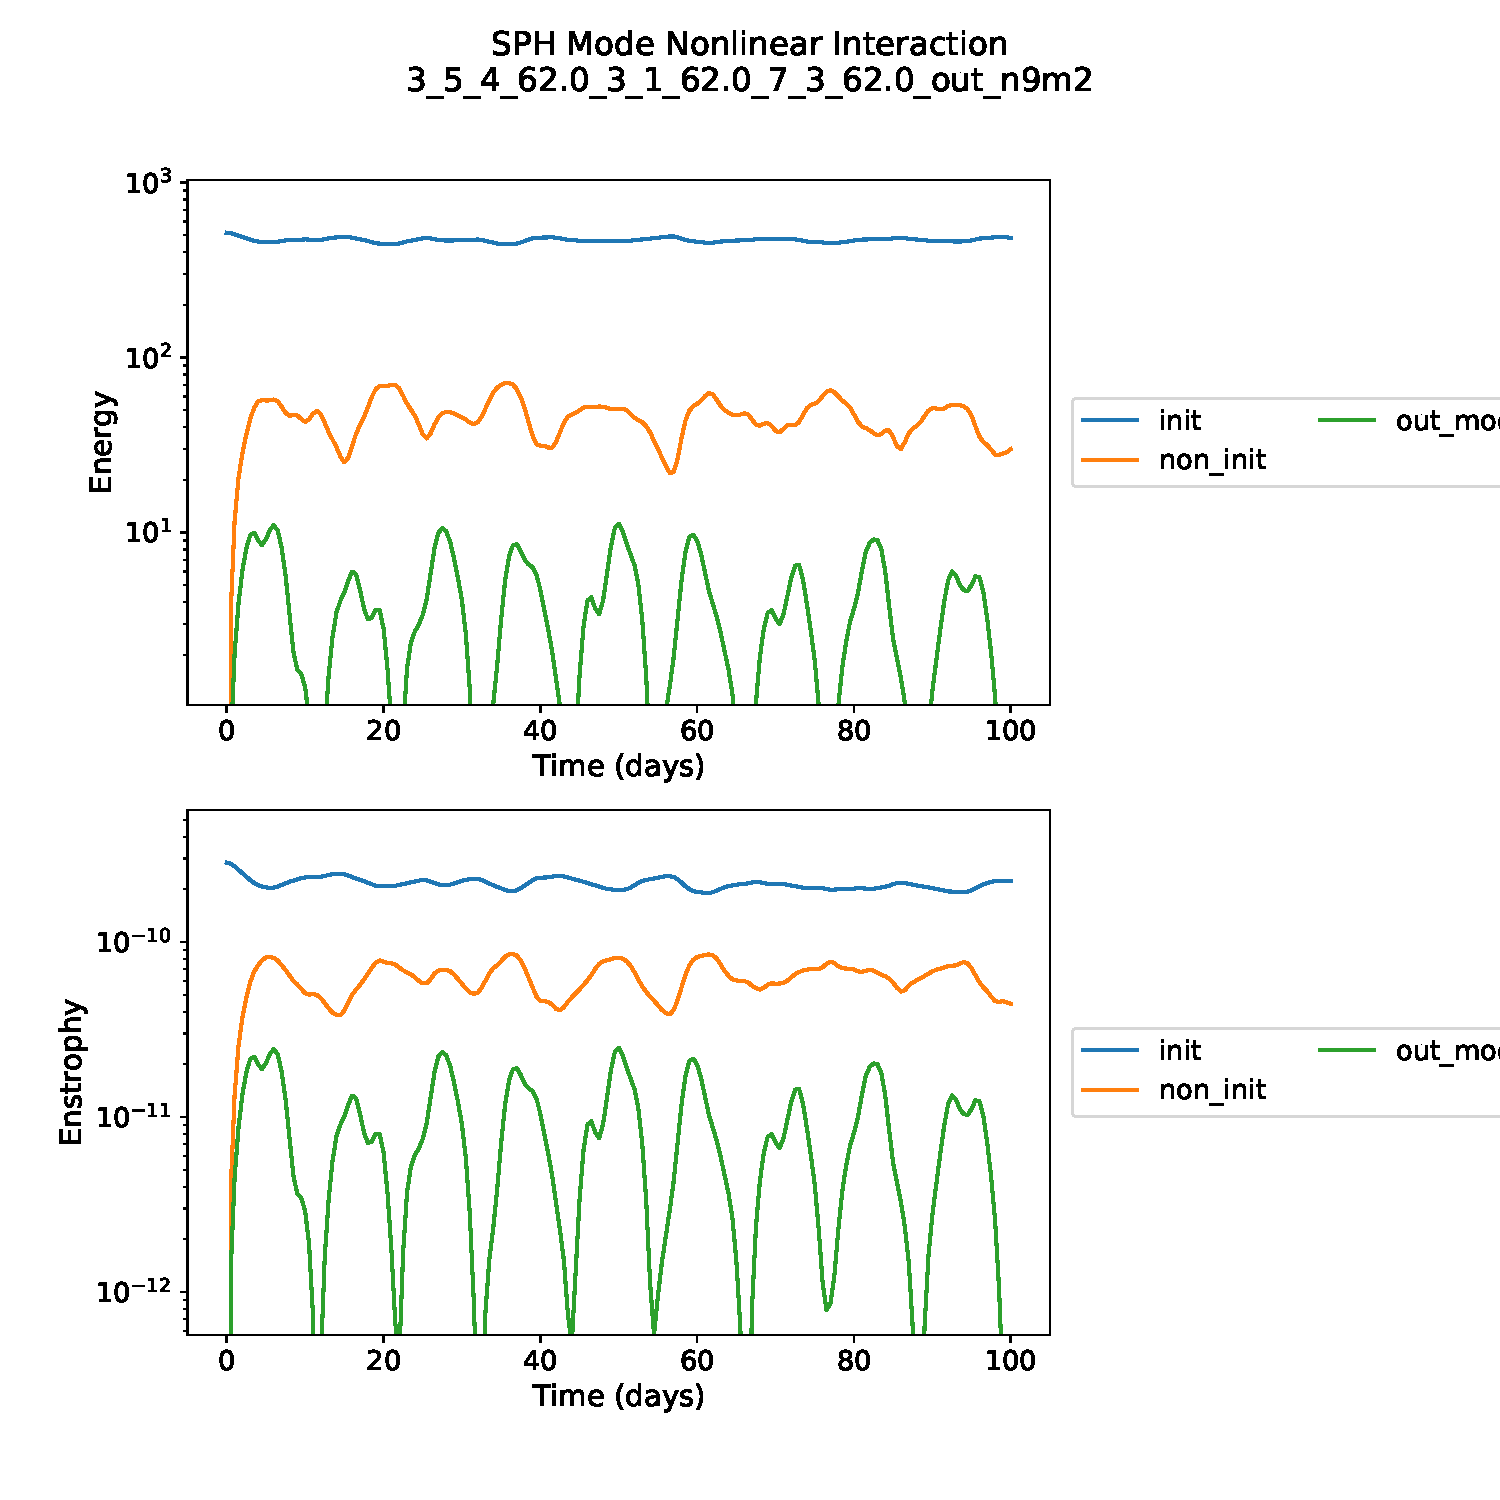
\includegraphics[scale=0.6]{figs/out_n9m2-alpha62.pdf}
 \label{tc2-alpha62}
 \caption{Evolution of energy in specific modes considering initial condition (init) with $\alpha=62$ on modes $(3,1)$, $(5,4)$, $(7,3)$. Non-init are all other modes not on initial condition and out-mode is mode $(9,2)$.}
\end{figure}

\begin{figure}
\centering
 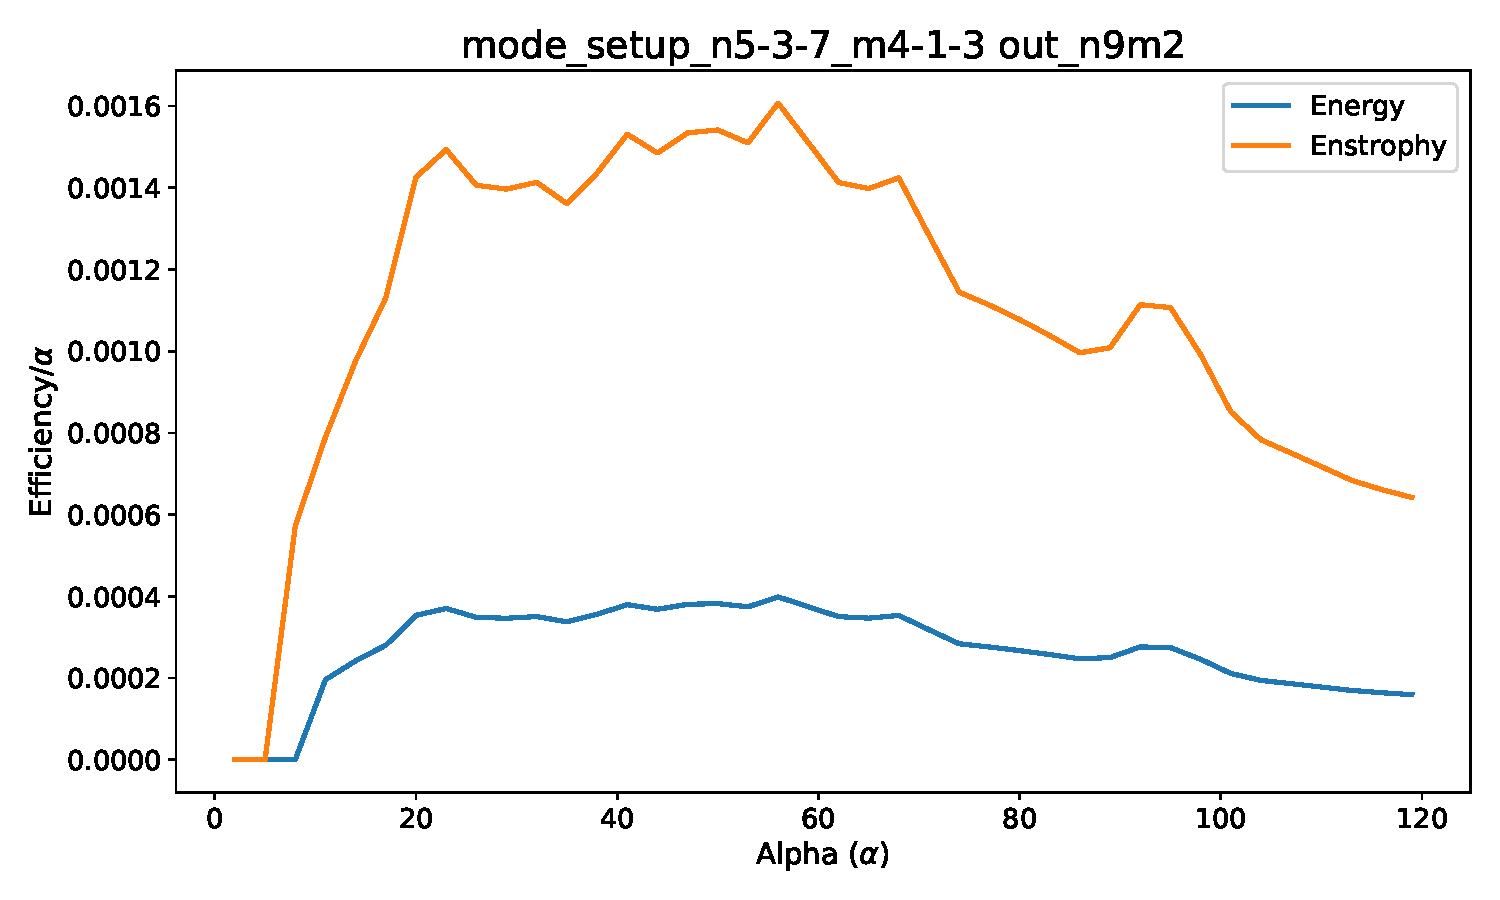
\includegraphics[scale=0.4]{figs/mode_setup_n5-3-7_m4-1-3_out_n9m2.pdf}
 \label{tc2-eficiency}
 \caption{Efficiency for test case with initial condition in modes modes $(3,1)$, $(5,4)$, $(7,3)$ monitoring the energy transfer to mode $(9,2)$.}
\end{figure}

\clearpage

\section{Test cases with background energy}

In preliminar experiments with the pervious 2 test cases but aditionally small amounts of energy on other modes show similar results.

\end{document}
